\documentclass{beamer}[10]

\usepackage{graphicx}
\usepackage{xcolor}
\usepackage{tabto}
%\usepackage{beamerthemesplit}
\usepackage{tikz}
\usepackage{cancel}
\usepackage{verbatim}
\usepackage{fancybox}
\usepackage{enumerate}
\usepackage{amsmath,amssymb,amsthm,textcomp,mathtools}
\usepackage[super]{nth}
\usepackage[amssymb]{SIunits}
\usepackage{booktabs}
\usepackage{cancel}
\usepackage{bm}
\usepackage[utf8]{inputenc}
\usepackage{tabularx}
\usepackage{ragged2e}
\newcolumntype{Y}{ >{\RaggedRight\arraybackslash}X}
\usetikzlibrary{arrows,shapes}
\newcommand\T{\rule{0pt}{2.6ex}}
\newcommand\B{\rule[-1.2ex]{0pt}{0pt}}
\definecolor{UUcrimson}{RGB}{204,0,0}
\mode<presentation>
{ \usetheme{default}
  \usecolortheme[named=UUcrimson]{structure}
  \useinnertheme{circles}
  \setbeamercovered{transparent}
  \setbeamertemplate{blocks}[rounded]
  \usefonttheme[onlymath]{serif}
  \setbeamertemplate{navigation symbols}{}
  \setbeamertemplate{footline}[page number]
  \setbeamertemplate{navigation symbols}{}
  \setbeamercolor{section in toc}{fg=black,bg=white}
  \setbeamercolor{alerted text}{fg=UUcrimson!80!gray}
  \setbeamercolor*{palette primary}{fg=white,bg=UUcrimson}
  \setbeamercolor*{palette secondary}{fg=UUcrimson!70!black,bg=gray!15!white}
  \setbeamercolor*{palette tertiary}{bg=UUcrimson!80!black,fg=gray!10!white}
  \setbeamercolor*{palette quaternary}{fg=UUcrimson,bg=gray!5!white}
  \setbeamercolor*{palette sidebar primary}{fg=UUcrimson!10!black}
  \setbeamercolor*{palette sidebar secondary}{fg=white}
  \setbeamercolor*{palette sidebar tertiary}{fg=UUcrimson!50!black}
  \setbeamercolor*{palette sidebar quaternary}{fg=gray!10!white}
  \setbeamercolor{titlelike}{parent=palette primary,fg=white}
  \setbeamercolor{frametitle}{bg=UUcrimson}
  \setbeamercolor{frametitle right}{bg=UUcrimson}
  \setbeamercolor*{separation line}{}
  \setbeamercolor*{fine separation line}{}
}

\usetikzlibrary{backgrounds}
\makeatletter
\tikzstyle{every picture}+=[remember picture]
\tikzset{%
  fancy quotes/.style={
    text width=\fq@width pt,
    align=justify,
    inner sep=1em,
    anchor=north west,
    minimum width=\linewidth,
    font=\itshape
  },
  fancy quotes width/.initial={.8\linewidth},
  fancy quotes marks/.style={
    scale=8,
    text=white,
    inner sep=0pt,
  },
  fancy quotes opening/.style={
    fancy quotes marks,
  },
  fancy quotes closing/.style={
    fancy quotes marks,
  },
  fancy quotes background/.style={
    show background rectangle,
    inner frame xsep=0pt,
    background rectangle/.style={
      fill=gray!25,
      rounded corners,
    },
  }
}
\newenvironment{fancyquotes}[1][]{%
\noindent
\tikzpicture[fancy quotes background]
\node[fancy quotes opening,anchor=north west] (fq@ul) at (0,0) {``};
\tikz@scan@one@point\pgfutil@firstofone(fq@ul.east)
\pgfmathsetmacro{\fq@width}{\linewidth - 2*\pgf@x}
\node[fancy quotes,#1] (fq@txt) at (fq@ul.north west) \bgroup}
{\egroup;
\node[overlay,fancy quotes closing,anchor=east] at (fq@txt.south east) {''};
\endtikzpicture}
\makeatother


\usetikzlibrary{backgrounds}
\makeatletter
\tikzstyle{every picture}+=[remember picture]
\tikzset{%
  fancy defs/.style={
    text width=\fq@width pt,
    align=justify,
    inner sep=0.25em,
    anchor=north west,
    minimum width=\linewidth,
    font=\itshape
  },
  fancy defs width/.initial={.8\linewidth},
  fancy defs marks/.style={
    scale=8,
    text=white,
    inner sep=0pt,
  },
  fancy defs opening/.style={
    fancy defs marks,
  },
  fancy defs closing/.style={
    fancy defs marks,
  },
  fancy defs background/.style={
    show background rectangle,
    inner frame xsep=0pt,
    background rectangle/.style={
      fill=gray!25,
      rounded corners,
    },
  }
}
\newenvironment{fancydefs}[1][]{%
\noindent
\tikzpicture[fancy defs background]
\node[fancy defs opening,anchor=north west] (fq@ul) at (0,0) {};
\tikz@scan@one@point\pgfutil@firstofone(fq@ul.east)
\pgfmathsetmacro{\fq@width}{\linewidth - 2*\pgf@x}
\node[fancy defs,#1] (fq@txt) at (fq@ul.north west) \bgroup}
{\egroup;
\node[overlay,fancy defs closing,anchor=east] at (fq@txt.south east) {};
\endtikzpicture}
\makeatother
\usepackage{scalerel}[2014/03/10]
\usepackage{stackengine}
\usepackage{empheq}
\newcommand*\widefbox[1]{\fbox{\hspace{0.5em}#1\hspace{0.5em}}}

\newcommand\reallywidetilde[1]{\ThisStyle{%
  \setbox0=\hbox{$\SavedStyle#1$}%
  \stackengine{-.1\LMpt}{$\SavedStyle#1$}{%
    \stretchto{\scaleto{\SavedStyle\mkern.2mu\sim}{.5467\wd0}}{.4\ht0}%
%    .2mu is the kern imbalance when clipping white space
%    .5467++++ is \ht/[kerned \wd] aspect ratio for \sim glyph
  }{O}{c}{F}{T}{S}%
}}
\usepackage{media9}

\logo{
\includegraphics[width=0.75cm]{logo.jpg}}
\author[Gibbs]{Dr. Jeremy A. Gibbs}
\institute{Department of Mechanical Engineering\\University of Utah}
\date{Spring 2017}
\title{Environmental Fluid Dynamics: Lecture 13}
% colors
\newcommand{\ihat}{\boldsymbol{\hat{\imath}}}
\newcommand{\jhat}{\boldsymbol{\hat{\jmath}}}
\newcommand{\khat}{\boldsymbol{\hat{k}}}
\definecolor{colororange}{HTML}{E65100} % orange
\definecolor{colordgray}{HTML}{795548} % dark gray for note
\definecolor{colorhgray}{HTML}{212121} % heavy dark gray for normal text
\definecolor{colorgreen}{HTML}{009688} % green
\definecolor{colorwhite}{HTML}{FFFFFF} % background white
\definecolor{colorlgray}{HTML}{F5F3EE} % background light gray
\definecolor{colorblue}{HTML}{0277BB} % blue
\definecolor{colorred}{HTML}{CC0000} % red
\newcommand{\fontsizeone}{1.9em}
\usepackage{esvect}
\setbeamertemplate{caption}{\raggedright\insertcaption\par}
\newcommand{\framecard}[2][colorgreen]{
  {\setbeamercolor{background canvas}{bg=#1}
    \begin{frame}[plain]
    \vfill
    \begin{center}
     {#2}
    \end{center}
    \vfill
    \end{frame}
  }
}
\begin{document}

%----------------------------------------------------------------------------------------
%	TITLE & TOC SLIDES
%----------------------------------------------------------------------------------------

\begin{frame} 
  \titlepage
\end{frame}

%------------------------------------------------

\begin{frame}
\frametitle{Overview}
\tableofcontents
\end{frame}

%------------------------------------------------
\section{Taylor-Proudman Theorem} %
%------------------------------------------------
\framecard[colorred]{{\color{white}\Huge Taylor-Proudman Theorem}}
%------------------------------------------------
\begin{frame}{Taylor-Proudman Theorem}

\begin{itemize}
	\item Consider the flow of a homogeneous flow that is in geostrophic balance.
	\item This flow is only observed in laboratory experiments because stratification effects cannot be avoided in nature.
	\item Imagine a tank with fluid that is steadily rotated at high angular speed $\Omega$.
	\item At the same time, a solid body is moved slowly across the bottom of the tank.
\end{itemize}
\end{frame}
%------------------------------------------------
\begin{frame}{Taylor-Proudman Theorem}

\begin{itemize}
	\item The angular speed $\Omega$ is made large, and the solid body is moved slowly, so that Coriolis $\gg$ acceleration terms.
	\item Acceleration terms must be negligible for geostrophic flow.
	\item Away from the frictional effects of the boundaries, the balance in this experiment is geostrophic in the horizontal and hydrostatic in the vertical.
	\begin{align}
		-2\Omega v &= -\frac{1}{\rho}\frac{\partial p}{\partial x} \label{eq1}\\
		2\Omega u &= -\frac{1}{\rho}\frac{\partial p}{\partial y}\label{eq2}\\
		0 &= -\frac{1}{\rho}\frac{\partial p}{\partial z} -g\label{eq3}
	\end{align}
\end{itemize}
\end{frame}

%------------------------------------------------
\begin{frame}{Taylor-Proudman Theorem}

\begin{itemize}
	\item Let's now define the Ekman number as the ratio of viscous to Coriolis forces (per unit volume):
	$$E = \frac{\rho\nu U/L^2}{\rho fU} = \frac{\nu}{fL^2}$$
	Based on the experimental setup, $E$ is very small.
\end{itemize}
\end{frame}

%------------------------------------------------
\begin{frame}{Taylor-Proudman Theorem}

\begin{itemize}
	\item First take $\partial/\partial y$ of Eq.~(\ref{eq1}):
	$$-2\Omega \frac{\partial v}{\partial y} = -\frac{1}{\rho}\frac{\partial}{\partial y}\frac{\partial p}{\partial x} = -\frac{1}{\rho}\frac{\partial}{\partial x}\frac{\partial p}{\partial y}$$
	\item Next take $\partial/\partial x$ of Eq.~(\ref{eq2}):
	$$2\Omega \frac{\partial u}{\partial x} = -\frac{1}{\rho}\frac{\partial}{\partial x}\frac{\partial p}{\partial y}$$
	\item Both equations are equal:
	$$-2\Omega \frac{\partial v}{\partial y} = 2\Omega \frac{\partial u}{\partial x}\rightarrow 2\Omega\left(\frac{\partial u}{\partial x} + \frac{\partial v}{\partial y}\right) = 0$$
	\item Recall that the incompressibility condition says $\vv{\nabla}\cdot\vv{U}=0$. Therefore, $\partial w/\partial z = 0$.
\end{itemize}
\end{frame}

%------------------------------------------------
\begin{frame}{Taylor-Proudman Theorem}

\begin{itemize}
	\item Next, differentiate Eqs.~(\ref{eq1}) and (\ref{eq2}) with respect to $z$:
	\begin{align*}
		-2\Omega \frac{\partial v}{\partial z} &= -\frac{1}{\rho}\frac{\partial}{\partial z}\frac{\partial p}{\partial x} = -\frac{1}{\rho}\frac{\partial}{\partial x}\frac{\partial p}{\partial z}\\
		2\Omega \frac{\partial u}{\partial z} &= -\frac{1}{\rho}\frac{\partial}{\partial z}\frac{\partial p}{\partial y} = -\frac{1}{\rho}\frac{\partial}{\partial y}\frac{\partial p}{\partial z}
	\end{align*}
	\item Using Eq.~(\ref{eq3}):
	$$
		-2\Omega \frac{\partial v}{\partial z} = \frac{\partial g}{\partial x} = 0 \qquad 
		2\Omega \frac{\partial u}{\partial z} = \frac{\partial g}{\partial y} = 0
	$$
	\item Both equations are equal:
	$$2\Omega \frac{\partial v}{\partial z} = 2\Omega \frac{\partial u}{\partial z} \rightarrow \frac{\partial u}{\partial z} = \frac{\partial v}{\partial z} = 0$$
	\item We already showed that $\partial w/\partial z=0$, so
	$$\frac{\partial \vv{U}}{\partial z} = 0$$
\end{itemize}
\end{frame}

%------------------------------------------------
\begin{frame}{Taylor-Proudman Theorem}
$$\frac{\partial \vv{U}}{\partial z} = 0$$
\begin{itemize}
	\item This outcome shows that the velocity vector does not vary in the direction of the $\vv{\Omega}$.
	\item In other words, steady, slow motions in a rotating, inviscid, homogeneous fluid are two-dimensional.
	\item This is the \textbf{Taylor-Proudman theorem}.
	\item This theorem was derived by Proudman in 1916 and proved experimentally by Taylor soon thereafter.
\end{itemize}
\end{frame}

%------------------------------------------------
\begin{frame}{Taylor-Proudman Theorem}
\setlength{\fboxsep}{0pt}
\setlength{\fboxrule}{1pt}
\begin{columns}[T]
    \begin{column}{.5\textwidth}
    	Taylor's Experiment:
    	\begin{itemize}
    		\item Dye was released at point A, above the cylinder.
    		\item If non-rotating, the dye would pass over the cylinder.
    		\item If rotating, the dye split at point S, as if blocked by an extension of the cylinder, and flowed around this imaginary column.
    		\item This was called a \textbf{Taylor column}.
    	\end{itemize}	
    \end{column}
    \begin{column}{.5\textwidth}
    	\begin{minipage}[c][.65\textheight][c]{\linewidth}
    		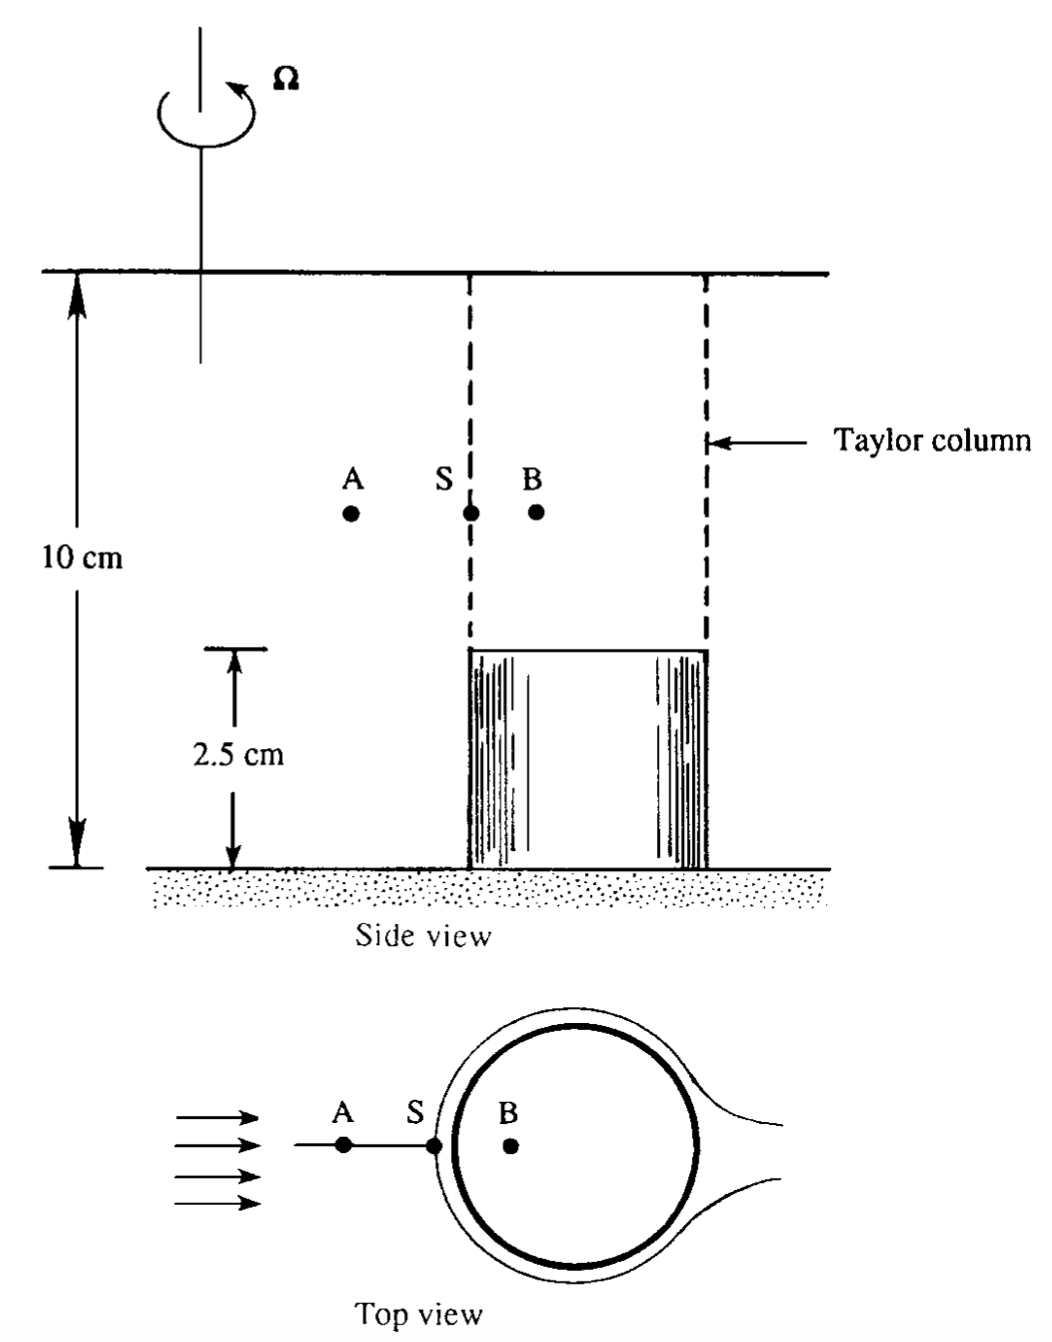
\includegraphics[width=\textwidth]{tp1}
    		\centering \tiny{~\\via: Kundu et al. (2008)}
    	\end{minipage}
    \end{column}
  \end{columns}
\end{frame}
%------------------------------------------------
\begin{frame}{Taylor-Proudman Theorem}
\setlength{\fboxsep}{0pt}
\setlength{\fboxrule}{1pt}
\begin{columns}[T]
    \begin{column}{.5\textwidth}
    	Taylor's Experiment:
    	\begin{itemize}
    		\item Dye released at point $B$ moved with the  cylinder.
    		\item Conclusion: the flow outside of the vertical extension of the cylinder was the same as if the cylinder extended across the entire water depth.
    		\item Conclusion: a column of water directly above the cylinder moved with it. 
    	\end{itemize}	
    \end{column}
    \begin{column}{.5\textwidth}
    	\begin{minipage}[c][.65\textheight][c]{\linewidth}
    		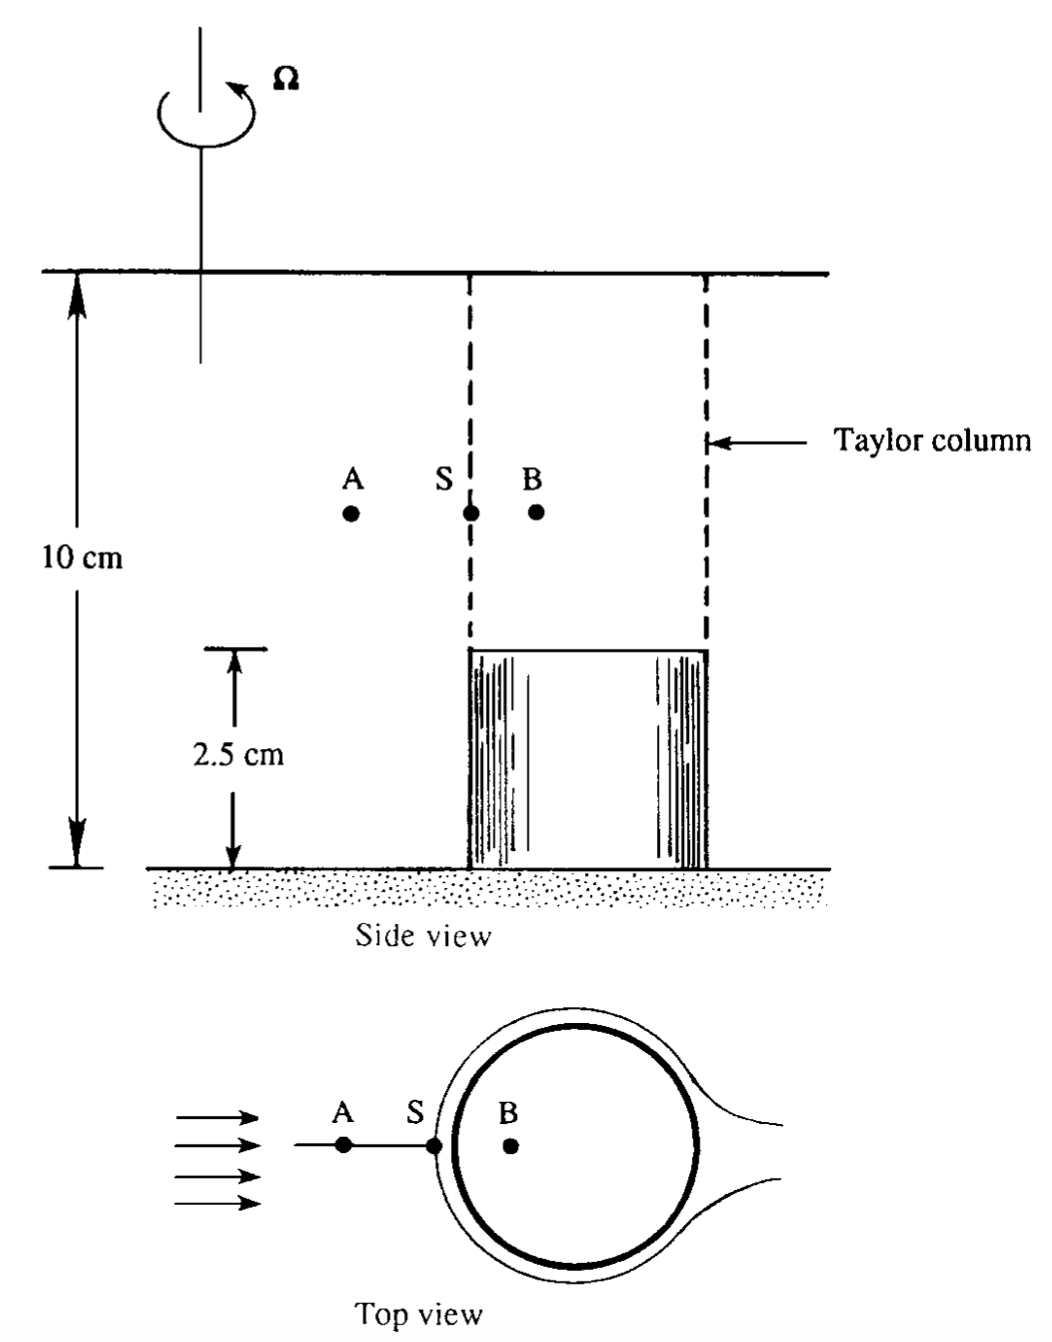
\includegraphics[width=\textwidth]{tp1}
    		\centering \tiny{~\\via: Kundu et al. (2008)}
    	\end{minipage}
    \end{column}
  \end{columns}
\end{frame}
%------------------------------------------------
\begin{frame}{Taylor-Proudman Theorem}
\begin{itemize}
	\item For the case of a rotating steady, inviscid, homogeneous fluid, Taylor's experiments showed that bodies moving parallel or perpendicular to the axis of rotation carry with them a Taylor column of fluid.
	\item This Taylor column of fluid is oriented parallel to the axis of rotation.
	\item This phenomenon is similar to horizontal solid-body blocking in the real (stratified) world, such as flow encountering a mountain.
\end{itemize}
\end{frame}
%------------------------------------------------
\section{Thermal Wind} %
%------------------------------------------------
\framecard[colorred]{{\color{white}\Huge Thermal Wind}}
%------------------------------------------------
\begin{frame}{Thermal Wind}

\begin{itemize}
	\item Recall that the geostrophic wind is:
	$$\vv{V_g} = \frac{1}{\rho f}\hat k \times \vv{\nabla} p$$
	\item We now define the \textbf{thermal wind} as:
	$$\vv{V_T} = \vv{V_g}_{\text{, upper}} -  \vv{V_g}_{\text{, lower}}$$
	\item The thermal wind is the vector difference between the geostrophic wind at some upper level and lower level.
	\item The name is a misnomer because it is not a wind.
\end{itemize}
\end{frame}
%------------------------------------------------
\begin{frame}{Thermal Wind}

\begin{itemize}
	\item Why do we care about vertical changes in the geostrophic wind?
	\item Vertical changes in $\vv{V_g}$ (and hence the thermal wind) are associated with horizontal changes in temperature.
	\item Recall that the hydrostatic balance is given by:
	$$\frac{\partial p}{\partial z} = -\rho g$$
	we can apply the ideal gas law $p=\rho R T$ to get:
	$$\frac{\partial p}{\partial z} = -\frac{pg}{RT}$$
\end{itemize}
\end{frame}
%------------------------------------------------
\begin{frame}{Thermal Wind}

\begin{itemize}
	\item Consider an infinitesimally small difference in height $\delta z$ between two adjacent pressure levels that are separated by the very small pressure difference $\delta p$:
	$$\delta z = -\frac{RT}{pg}\delta p$$
	\item Integrate to get the thickness between these two pressure levels spaced arbitrarily far apart:
	$$z_2 - z_1 = -\frac{R}{g}\int^{p_2}_{p1} \frac{T}{p} dp$$
	\item Thus, the thickness of a layer is proportional to the temperature in the layer.
\end{itemize}
\end{frame}
%------------------------------------------------
\begin{frame}{Thermal Wind}

\begin{itemize}
	\item As an example:
	\begin{figure}
		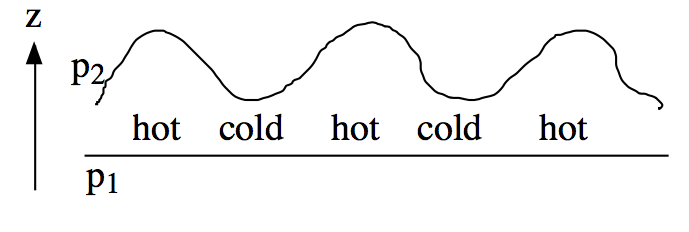
\includegraphics[width=0.75\textwidth]{thermal1}
	\end{figure}
	\item Another example with the same temperature field:
	\begin{figure}
		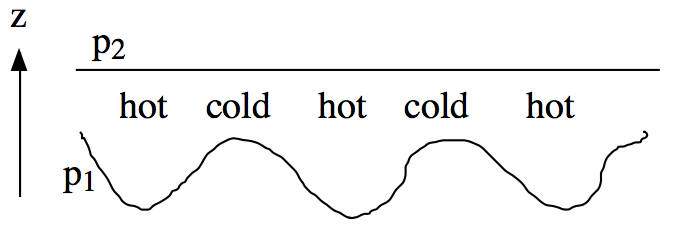
\includegraphics[width=0.75\textwidth]{thermal2}
	\end{figure}
	\item In both cases, the geostrophic wind changes with height because of horizontal temperature gradients.
\end{itemize}
\end{frame}
%------------------------------------------------
\begin{frame}{Thermal Wind}

\begin{itemize}
	\item The expression for the thermal wind is messy!
	$$\vv{V_T} = \vv{V_g}_{\text{, upper}} -  \vv{V_g}_{\text{, lower}} = \frac{1}{\rho_{f \text{upper}}}\hat k \times \vv{\nabla} p_{\text{upper}} - \frac{1}{f \rho_{\text{upper}}}\hat k \times \vv{\nabla} p_{\text{lower}}$$
	\item We can make life easier if we switch to isobaric coordinates by using
	$$\frac{1}{\rho}\vv{\nabla}_z p = \vv{\nabla}_p \Phi$$
	where $\Phi = gz$. We get a much nicer expression:
	$$\vv{V_T} = \frac{1}{f} \times \vv{\nabla}_p \left(\Phi_{\text{upper}} - \Phi_{\text{lower}}\right)$$
\end{itemize}
\end{frame}
%------------------------------------------------
\begin{frame}{Thermal Wind}

\begin{itemize}
	\item Remember that the thermal wind is related to the vertical shear of the geostrophic wind:
	\begin{align*}
	\vv{V_g} &= \frac{1}{f} \hat k \times \vv{\nabla}_p \Phi \qquad{\text{take $\partial/\partial p$}}\\
	\frac{\partial \vv{V_g}}{\partial p} &= \frac{1}{f} \hat k \times \vv{\nabla}_p \frac{\partial \Phi}{\partial p}
	\end{align*}
\hrule
$$\frac{\partial p}{\partial z} = -\rho g \rightarrow \text{[$\div$ by $g$ and use $gz=\Phi$]} \rightarrow \frac{\partial p}{\partial \Phi} = -\rho$$
$$\frac{\partial \Phi}{\partial p} = -\frac{1}{\rho} \rightarrow [\text{use ideal gas law}] \rightarrow \frac{\partial \Phi}{\partial p} = -\frac{RT}{p}$$
We've now related $\partial \Phi/\partial p$ to $T$
~\\~\\
\hrule
\end{itemize}
\end{frame}
%------------------------------------------------
\begin{frame}{Thermal Wind}

\begin{itemize}
	\item Continuing:
	\begin{align*}
	\frac{\partial \vv{V_g}}{\partial p} &= \frac{1}{f} \hat k \times \vv{\nabla}_p \left(-\frac{RT}{p}\right)\quad \text{$p$=constant for isobaric level}\\
	\frac{\partial \vv{V_g}}{\partial p} &= -\frac{R}{fp} \hat k \times \vv{\nabla}_p T\\
	\Aboxed{-\frac{\partial \vv{V_g}}{\partial p} &= \frac{R}{fp} \hat k \times \vv{\nabla}_p T}
	\end{align*}
	This is the \textbf{thermal wind relation}, although it is really an equation for the vertical shear of the geostrophic wind.
\end{itemize}
\end{frame}
%------------------------------------------------
\begin{frame}{Thermal Wind}

\begin{itemize}
	\item Integrating the thermal wind relation will lead to the following general relationship in the Northern Hempisphere:
	$$\vv{V_T} = (\text{positive values})\hat k \times \vv{\nabla}_p T$$
	Thus, $\vv{V_T}$ is parallel to mean isotherms in a layer, with cold air to the left of $\vv{V_T}$.
	\begin{figure}
	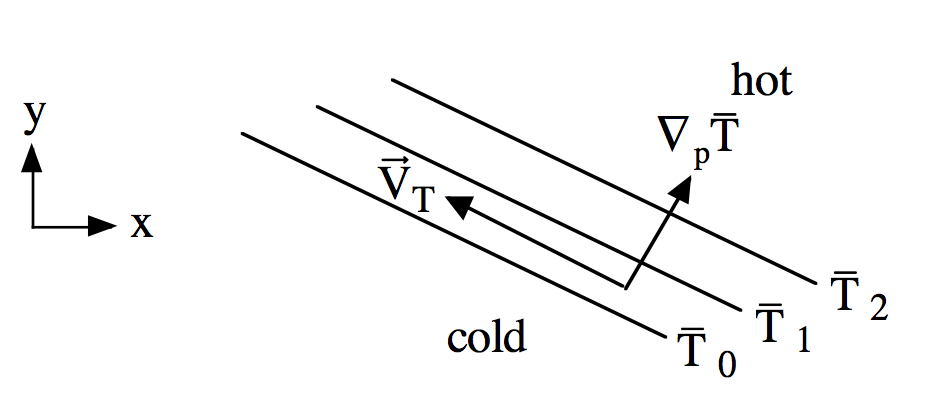
\includegraphics[width=0.5\textwidth]{thermal3}	
	\end{figure}
	\item This describes the \textbf{Thermal Buys-Ballot Law}: ``with $\vv{V_T}$ to your back, cold air is to your left.''
\end{itemize}
\end{frame}
%------------------------------------------------

\end{document}

